\cleardoublepage
\phantomsection
\stepcounter{chapter}
\label{chap:walkthrough}
\addcontentsline{toc}{chapter}{\protect\numberline{\thechapter}\acs{EsPy} Walkthroughs}
\chaptermark{\acs{EsPy} Walkthroughs}
% The remainder of this thesis is an insert from the documentation of
% version 2.0 of \acs{EsPy}. The section of the documentation included provides
% wlkthroughs describing how to use the package's \ac{API} for the consideration
% of \ac{1D} and \ac{2DJ} \ac{NMR} datasets \note{Sequential data too?}. These
% walkthroughs provide a short description of the key features associated with
% the package, and is an ideal first place to get up-and-running with using it.

\phantomsection
\stepcounter{section}
\addcontentsline{toc}{section}{\protect\numberline{\thesection}1D Walkthrough}
\sectionmark{1D Walkthrough}
\includepdf[%
    pages={13-19},%
    pagecommand={\thispagestyle{fancy}},%
    offset=0 -1cm,%
]{nmr-espy.pdf}

\phantomsection
\stepcounter{section}
\addcontentsline{toc}{section}{\protect\numberline{\thesection}2DJ Walkthrough}
\sectionmark{2DJ Walkthrough}
\includepdf[%
    pages={20-28},%
    pagecommand={\thispagestyle{fancy}},%
    offset=0 -1cm,%
]{nmr-espy.pdf}
